%!TEX encoding = UTF-8 Unicode
%!TEX root = ./../main.tex
%!TEX TS-program = xelatex

\chapter[OBP App.]{Observation Pack Approssimato} % chapter 6 title
\label{cap:sei}
L'obiettivo di questo lavoro è indagare la capacità di apprendere linguaggi regolari in uno scenario di \textit{Active Learning}, nel caso in cui non si disponga di un \textit{Oracolo} capace di rispondere nativamente nè ad \ac{EQ} nè a \ac{MQ}.  
In letteratura esistono diversi algoritmi utilizzati per  l'appredimento di linguaggi regolari. 
L' approssimazione dell' \textit{Oracolo} è  indipendente dallo specifico algoritmo d'\ac{IIR}, tuttavia per renderlo concreto l'attenzione è stata focalizzata sull'\ac{ObP}.
Allo stato dell'arte l' \ac{ObP} costituisce il secondo algoritmo di riferimento nell'ambito dell'apprendimento di linguaggi regolari.  L'algoritmo più performante è invece il più recente TTT algorithm \cite{SteffenTTT14}. Si è scelto di utilizzare \ac{SVM} come classificatore atto a modellare un \textit{Oracolo}, classificatore costruito a partire da alcuni esempi positivi e negativi del linguaggio da apprendere. Sarebbe opportuno preventivamente leggere le Appendici \ref{cap:cinque}  e \ref{app:tre} dato che i concetti e le tecniche lì descritte sono propedeudiche all'algoritmo qui delineato.\\
 Data la natura non esatta dell'algoritmo ivi realizzato questo viene indicato come \ac{ObPA}.\\
  Corredata a questa tesi vi è anche l'implementazione dell' \ac{ObP} in C++11 , codice che è stato integrato in  Gi-learning \cite{Cot16} una libreria preesistente. Nelle applicazioni reali tuttavia è altamente improbabile la disponibilità di un \textit{Oracolo} in grado di rispondere a delle \ac{EQ} da cui l'esigenza di un \textit{Oracolo approssimato} e dell'\ac{ObPA} la cui relativa implementazione oggetto di tesi è stata parimenti integrata in  Gi-learning \cite{Cot16}.

\section{Precedenti lavori in letteratura}
Assumere che il \textit{teacher} sia in possesso del formalismo del linguaggio target \ac{L} è uno scenario poco plausibile essendo esso stesso l'oggetto dell'inferenza.
Quindi l'obiettivo delineato in questa tesi è indagare il comportamento di un algoritmo di \textit{active learning} per inferire il \ac{DFA} A tale che $L(A) =\ac{L}$ tramite un oracolo approssimato realizzato con un classificatore statistico e tale intento si discosta dai lavori preesistenti in letteratura. In realtà una prima versione di un algoritmo di \textit{active learning} che realizza un Oracolo approssimato è già presente in Angluin \cite{Angluin87} in cui si approssima un \ac{EQ} tramite un certo numero di \ac{MQ} nella sua versione di L* approssimato. Più di recente, nella stessa direzione è andata la competizione Zulu \cite{Zulu10}: il vincitore della competizione \cite{Howar12} definisce il nuovo tipo di query: l'  \textit{Identity Query}
\begin{definizione*}[Identity Query] Testa se due prefissi $u,u'$ sono nella stessa classe di equivalenza del target A cioè se $u \not\simeq_{\lambda^{A}} \! u'$. In caso $u \not\simeq_{\lambda^{A}} \! u'$ ritorna un suffisso $v$ per il quale $\lambda^{A}(uv) \neq \lambda^{A}(u'v)$. Altrimenti ritorna il successo. 
\end{definizione*}
e dimostra che i linguaggi regolari possono essere inferiti con un numero polinomiale di \ac{MQ} ed \textit{Identity Query}.       
Le \textit{Identity Query} non sono meno realistiche delle \ac{EQ} ma forniscono un framework per organizzare le \ac{EQ} incrementalmente in modo da approssimarle in maniera relativamente facile ed efficiente tramite \ac{MQ}.  Anche gli altri algoritmi in letteratura sono focalizzati sulla ricerca di algoritmi che in maniera efficiente riescono ad approssimare le \ac{EQ} tramite \ac{MQ}.  In questa sede si assume invece l'impossibilità di rispondere nativamente anche alle \ac{MQ} oltre che alle \ac{EQ}, cioè  anche l'esito delle \ac{MQ} non è noto ed andrà approssimato.

Per quanto concerne la selezione del classificatore statistico per approssimare l'Oracolo la scelta è ricaduta su \ac{SVM} perchè costituiscono uno dei migliori modelli. Inoltre sono poche le applicazioni delle \ac{SVM} per l'apprendimento di linguaggi regolari come in \cite{Clark11}\cite{Clark06}  in cui si riesce a definire un kernel string utile per l'apprendimento dei linguaggi planari\footnote{I linguaggi planari sono una classe di linguaggi che attraversano la tassonomia di Chomsky nel senso che apprendono solo in maniera parziale i linguaggi finiti,regolari,context-free,context-sensitive ecc. senza saturare nessuno di essi}  oppure in \cite{Kontorovich09} dove si delinea un lavoro teorico sui linguaggi regolari e si propone un kernel string senza concretizzarlo specificamente per l'apprendimento di linguaggi regolari nell'accezione dell'\textit{active learning}. Altri tipi di classificatori come ad esempio le \textit{Recurrent Neural Network} si sono rilevate particolarmente adatte allo scopo di modellare un \ac{DFA} ma come si evince da \cite{Forcada02}, che costituisce una panoramica su di esse a riguardo dell'impiego in  \ac{GI}, sono state già ampiamente dibattute in letteratura.

\section{Funzionamento ObPA}
Una preliminare osservazione per evitare la creazione di ambiguità nel prosieguo consiste nel rimarcare che il codice prodotto è costituito da una duplice versione. Vi è infatti il codice riguardante la fase di \textit{debug} riferito d'ora in avanti come \textit{debug version} e quello pronto per l'utilizzo reale riferito d'ora in avanti come \textit{release version}\footnote{In realtà esiste un unica versione del codice ma si passa da una versione all'altra attivando o disattivando il flag in compilazione DEBUG$\_$EVALUATION (se è definito si sta optando per la \textit{debug version})}. La differenza principale tra le due versioni è che nella \textit{debug version} si è in possesso del \ac{DFA} target. Con l'intento di spiegare più in dettaglio le differenze tra le due versioni e contemporaneamente introdurre l'\ac{ObPA} vengono forniti gli pseudocodici \ref{alg:obpad} e \ref{alg:obpar} di alto livello:

\begin{algorithm}
\caption{OBPA \textit{debug version}}\label{alg:obpad}
\begin{algorithmic}[1]
\Statex
\Input il \ac{DFA} target $A$,l' alfabeto $\Sigma$ di $A$ 
\Output il \ac{DFA} inferito $Ob\_DFA$
\State $samples \gets A.random\_walk(750,750)$
\State $training\_set \gets pull\_out(samples,500)$
\State $test\_set \gets pull\_out(samples,1000)$
\State $appr\_oracle \gets \textbf{new}\:\: appr\_oracle(|\Sigma|,\Sigma,training\_set,test\_set)$
 \LineComment{Sul training\_set si addestra SVM e con il  \textit{test\_set} si fa model evaluation}
\State $Ob\_DFA \gets OBSERVATION\_PACK(appr\_oracle).run()$
\State $statistical\_measure \gets compare(Ob\_DFA , A)$
 \State \textbf{return} $Ob\_DFA$
     
\end{algorithmic}
\end{algorithm}





\section{ALtro}
Inserire il discorso che in debug version alla fine è comunque necessario confrontare l'ipotesi finale col target per rendersi conto del dfa inferito quanto è buono. Infatti che l'ipotesi sia verificato tramite un'equivalence query essere simile al classificatore non è sufficiente in quanto il classificatore è già di per sè un'approssimazione del target e quindi un'ipotesi che approssima bene il classificatore potrebbe non approssimare bene il target e quindi un confronto finale tra target e ipotesi è necessario. 

Inserire il discorso dell'esplosione del DFA. E che questo è dovuto anche al fatto che quando viene tornato un controesempio che non è un controesempio si fanno degli split errati. Siccome la versione implementata in librearia è ONEGlobally questa può generare più di uno split alla volta a differenza di ONELocally. Inoltre il controesempio viene sfruttato più di una volta, quindi anche un solo errore può condurre nel controesempio può condurre ad un DFA ipotesi completamente divergente dal target. Quindi potrebb essere meglio usare ONELocally che però è stato implementato ma non funzionava bene al 100 per 100.

Inserire il fatto che vengono generati due campioni di stringhe uno sull'ipotesi inferita e una sul target quando non è possibile usare il W-Method altrimenti no. 

LearnLib\footnote{\href{http://www.learnlib.de/}{http://www.learnlib.de/}}




\section{Scelte Progettuali}
Un lavoro d'implementazione degno di nota è costituito dalla preliminare ingegnerizzazione del codice. Come detto il prescelto algoritmo di \textit{active learning} è stato \ac{ObP}, che nella sua versione base presentata nel capitolo \ref{cap:quattro} necessita di un \ac{DFA} target che funge da Oracolo onnisciente. Nell'ottica di preservare questa versione dell'\ac{ObP} e contemporaneamente integrare nella libreria le funzionalità dell'\ac{ObPA} si è deciso di implementare una versione polimorfica. Più in dettaglio si è creata una gerarchia di classi per l'entità astratta Oracolo come in figura \ref{fig:eor}.
\begin{figure}[htp]
	\centering
	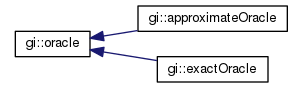
\includegraphics[ width=0.7\textwidth]{EreditaOracolo}
	\caption[Ereditarietà Oracolo]{Ereditarietà Oracolo}
   \label{fig:eor}
\end{figure}

L'algoritmo \ac{ObP} invece di possedere (composizione) un \ac{DFA} target ha un oggetto della classe base astratta Oracolo. Quando invoco il costruttore dell' \ac{ObP}  si deve passare anche l'indirizzo di un oggetto della classe Oracolo. Tramite il tipo di oggetto Oracolo(si ha un handle della classe base Oracolo che punta allo specifico oggetto della classe derivata passato) passato  viene determinato in maniera trasparente con il polimorfismo se si desidera utilizzare l'\ac{ObP} piuttosto che l'\ac{ObPA}. Le chiamate alle funzioni effettuate sull'oggetto Oracolo all'interno di \ac{ObP} hanno la stessa \textit{signature} , cioè le \ac{MQ} e le \ac{EQ} , ma il tipo dell'oggetto Oracolo passato determina automaticamente di quale classe derivata invocare le funzioni (che avranno diverse implementazioni a secondo se appartengono alla classe exactOracle o a quella approximateOracle).  In questo modo la classe dell'algoritmo \ac{ObP} ha subito pochissime modifiche  e il lavoro d'implementazione di questa tesi si è focalizzato sulla classe approximateOracle. Infine all'interno della classe observation\_pack , per impedire al \textit{client} di vedere le strutture dati e le modifiche effettuate su di esse  e in ultimo il modo in cui funziona l'algoritmo, è necessario effettuare una copia interna dell'Oracolo passato dal \textit{client} ma non conoscendo a priori di quale tipo, e quindi di quale classe, è l'Oracolo vi è stata la difficoltà su come invocare il costruttore di copia. A tal fine si è usata la tecnica del \textit{clone idiom} .Quando si ha un riferimento polimorfico cioè un 
  puntatore alla classe base che punta a un oggetto della classe derivata all'occorrenza può sorgere il problema di determinare qual è il tipo della classe derivata . Allora nella classe base si dichiara un metodo virtuale puro che tutte le classi derivate devono quindi implementare. Quest'implementazione consiste nella creazione dinamica  di un nuovo oggetto della classe derivata chiamando il costruttore di copia della classe derivata sull'oggetto corrente (tramite new classeDerivata(*this)). Questo nuovo oggetto creato verrà tornato al chiamante. Si noti che il costruttore di copia della classe derivata deve provvedere a chiamare il costruttore di copia della classe base e che in questi costruttori deve avvenire una deep copy di tutti i membri dinamici.   In figura \ref{fig:cba} l'interfaccia della classe base astratta.
  
 \begin{figure}[htp]
	\centering
	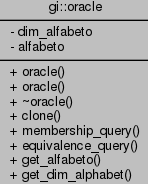
\includegraphics[ width=0.3\textwidth]{Oracolo}
	\caption[Interfaccia classe base Oracolo]{Interfaccia classe base Oracolo}
   \label{fig:cba}
\end{figure}    